\chapter{Inicio de la Aplicación}

\section{Pantalla Principal}

La aplicación \textit{MDAA} ofrece una interfaz moderna y adaptable. Al acceder a la página de inicio por primera vez, se presenta la vista por defecto de la aplicación. Esta pantalla es el punto de partida y de bienvenida al entorno de trabajo.

\begin{figure}[!ht]
    \centering
    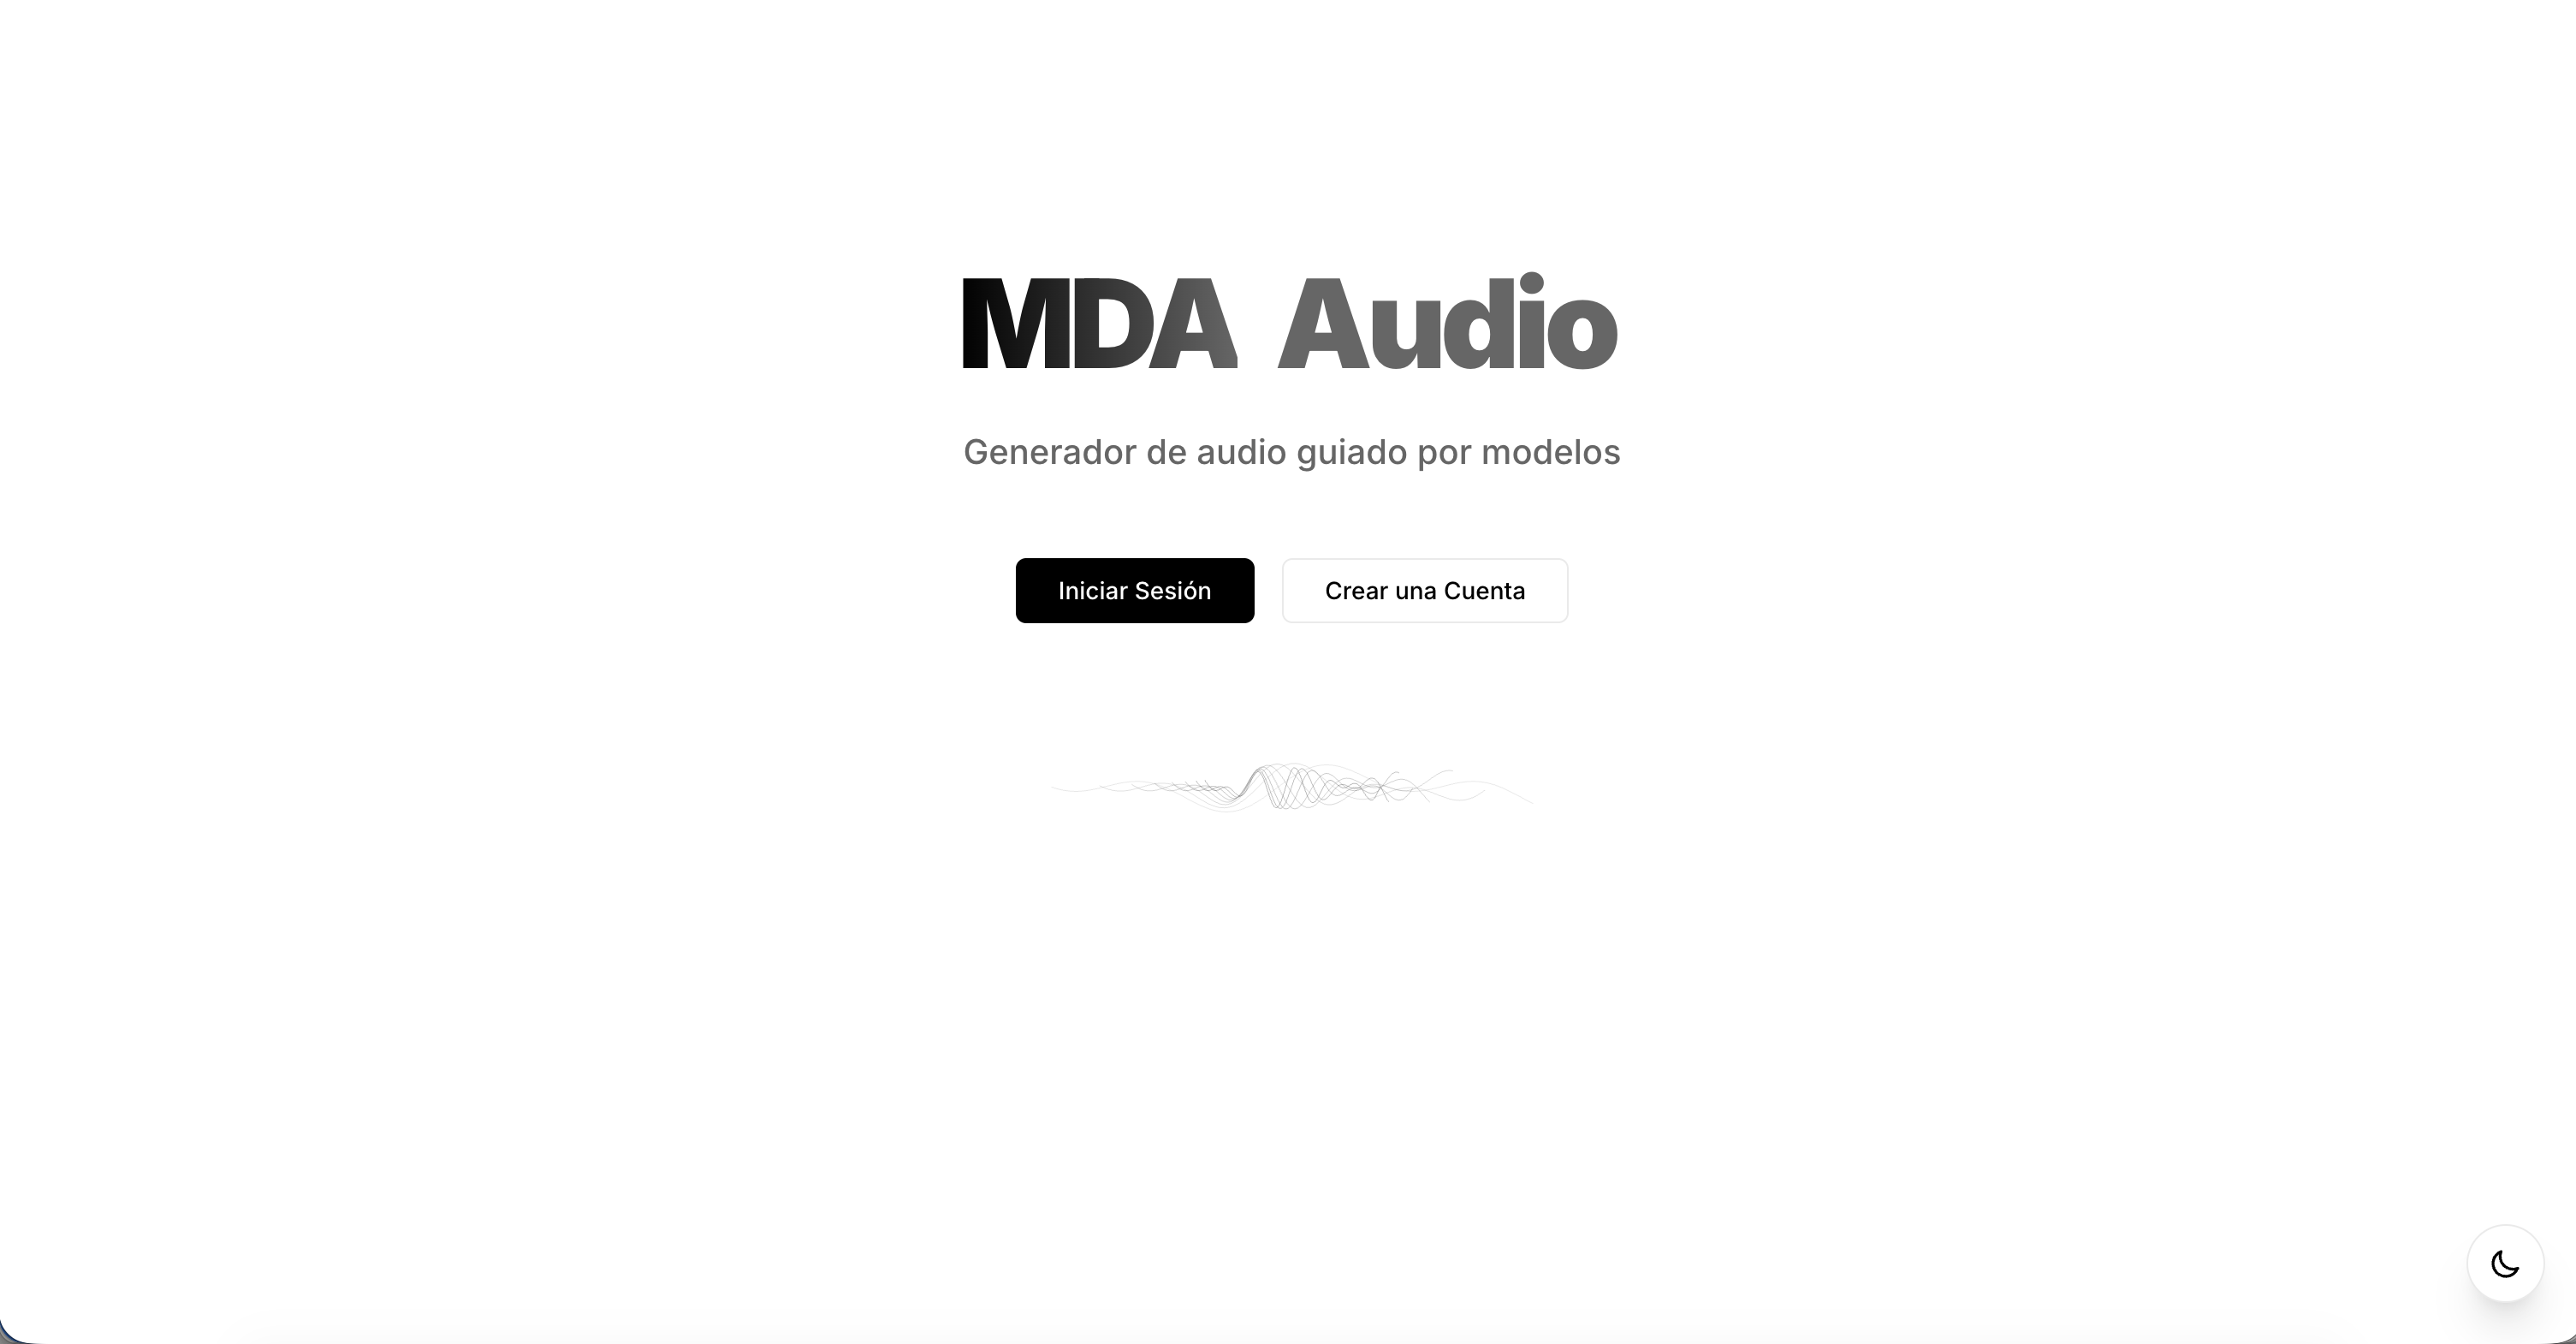
\includegraphics[width=\textwidth]{imagenes/01_inicio/01_pantallaInicioBlanca.png}
    \caption{Pantalla de inicio en tema claro.}
\end{figure}

Esta interfaz muestra una disposición limpia, diseñada para orientar rápidamente al usuario sobre las capacidades del sistema. Las opciones disponibles en esta vista inicial son:

\begin{itemize}
    \item \textbf{Barra de navegación superior:} Contiene el título de la aplicación y botones de acceso rápido para iniciar sesión o registrarse en el sistema.
    \item \textbf{Área de contenido principal:} Muestra información introductoria y llamadas a la acción para comenzar a trabajar con los modelos \textit{CIM} y \textit{PIM}.
\end{itemize}

\begin{figure}[!ht]
    \centering
    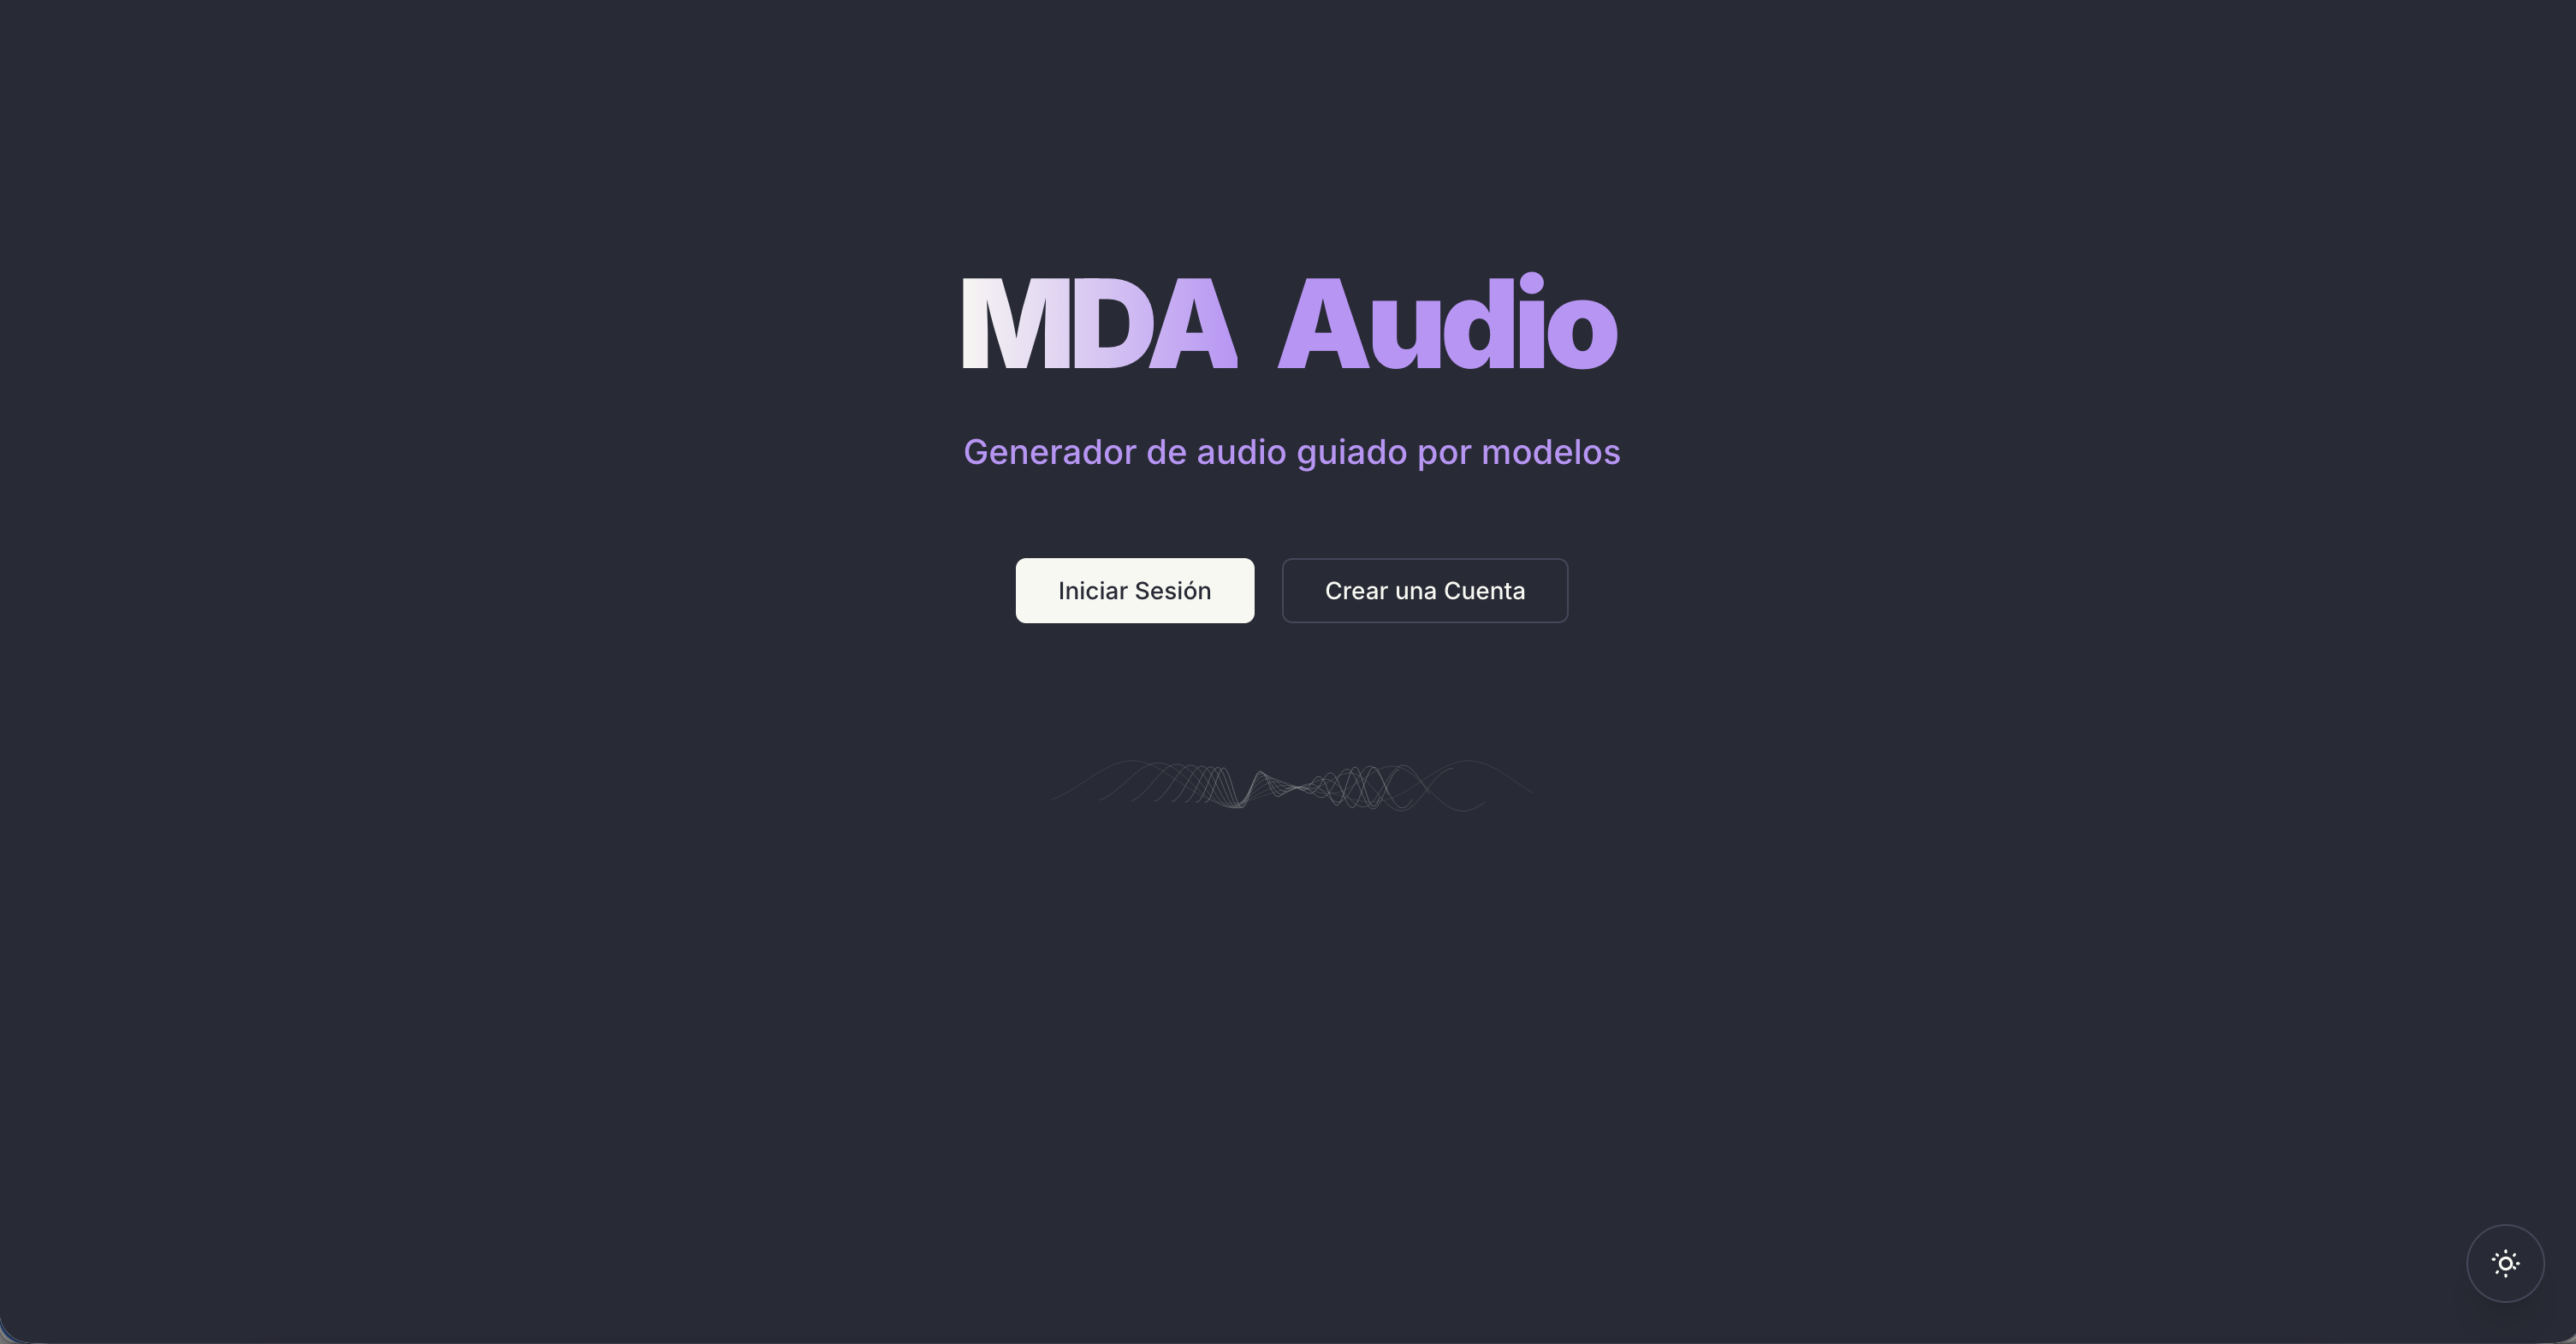
\includegraphics[width=\textwidth]{imagenes/01_inicio/02_pantallaInicioOscura.png}
    \caption{Pantalla de inicio en tema oscuro.}
\end{figure}

La aplicación soporta de forma nativa la alternancia de temas. El tema oscuro reduce la fatiga visual y puede ser activado según las preferencias del sistema operativo del usuario. Las funcionalidades, accesos y opciones de la pantalla son completamente idénticas a las del tema claro.
